\section{Forces on a 2-dimensional body}

With the Bernoulli equation, 
\begin{equation}
\vec{\nabla}\left(\frac{\rho}{2}\vec{u}^2+p\right)=0.
\end{equation}
we can calculate the force on the "obstacle" (\fref{fig:2dim-body}) from the surrounding flow:
\begin{align}
\vec{F} &= \int_{S}(-p(\vec{r}))d\vec{A} = -\int_{S}\left(p_0-\frac{\rho}{2}\vec{u}^2(\vec{r})\right)d\vec{A} \\
&= \frac{\rho}{2}\int_{S}\vec{u}^2(\vec{r})d\vec{A}\\
&= L\vec{e}_y +\underbrace{D\vec{e}_x}_{=0}.
\end{align}
$\vec{L}$ is the lift force and $\vec{D}$ is the drag force. The last term equals zero because there is no friction in ideal flows.

\begin{figure}[!h]
    \centering
    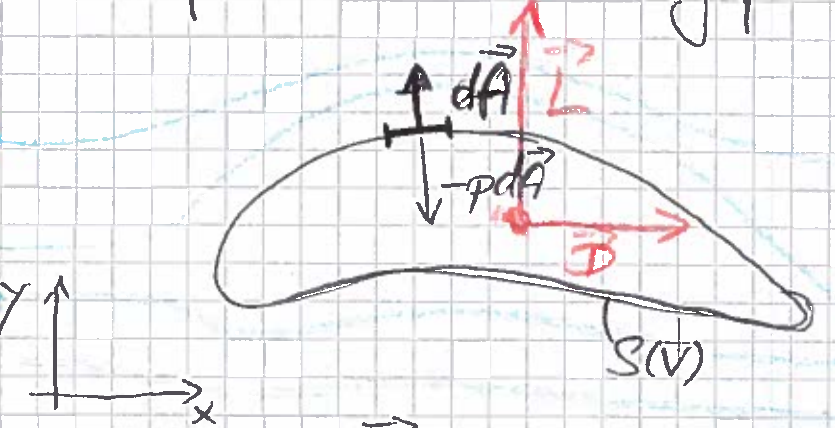
\includegraphics[width=.5\textwidth]{week4/2dim-body}\\
    \caption{Lift and drag forces.}
    \label{fig:2dim-body}
\end{figure}

\begin{figure}[!h]
    \centering
    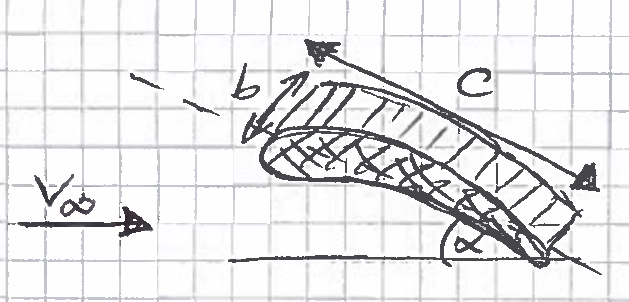
\includegraphics[width=.4\textwidth]{week4/generic-lift2}\\
    \caption{Angle of attack.}
    \label{fig:generic-lift2}
\end{figure}

Lift coefficient
\begin{equation}
C_L = \frac{L}{\frac{\rho}{2}v_\infty^2 b c}
\end{equation}
Drag coefficient (for the case that friction is non-zero):
\begin{equation}
C_D = \frac{D}{\frac{\rho}{2}v_\infty^2 b c}
\end{equation}

\begin{figure}[!h]
    \centering
    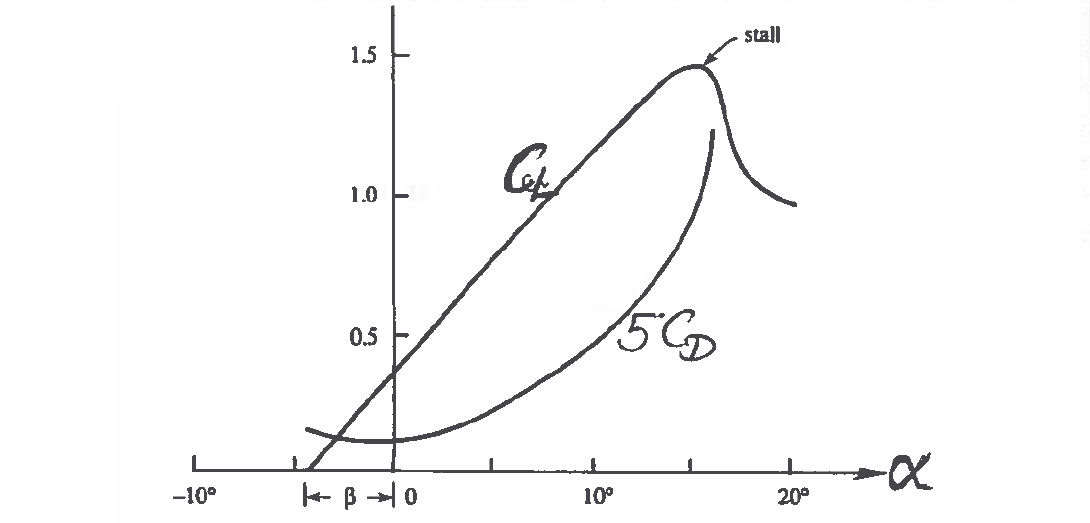
\includegraphics[width=.5\textwidth]{week4/generic-lift}\\
    \caption{Generic lift and drag coefficients vs. angle of attack.}
    \label{fig:generic-lift}
\end{figure}


\subsection{Turbine blade}
The lift force pulls the rotor blade of a wind turbine forward. See \fref{fig:turbine-blade}.
\begin{figure}[!h]
    \centering
    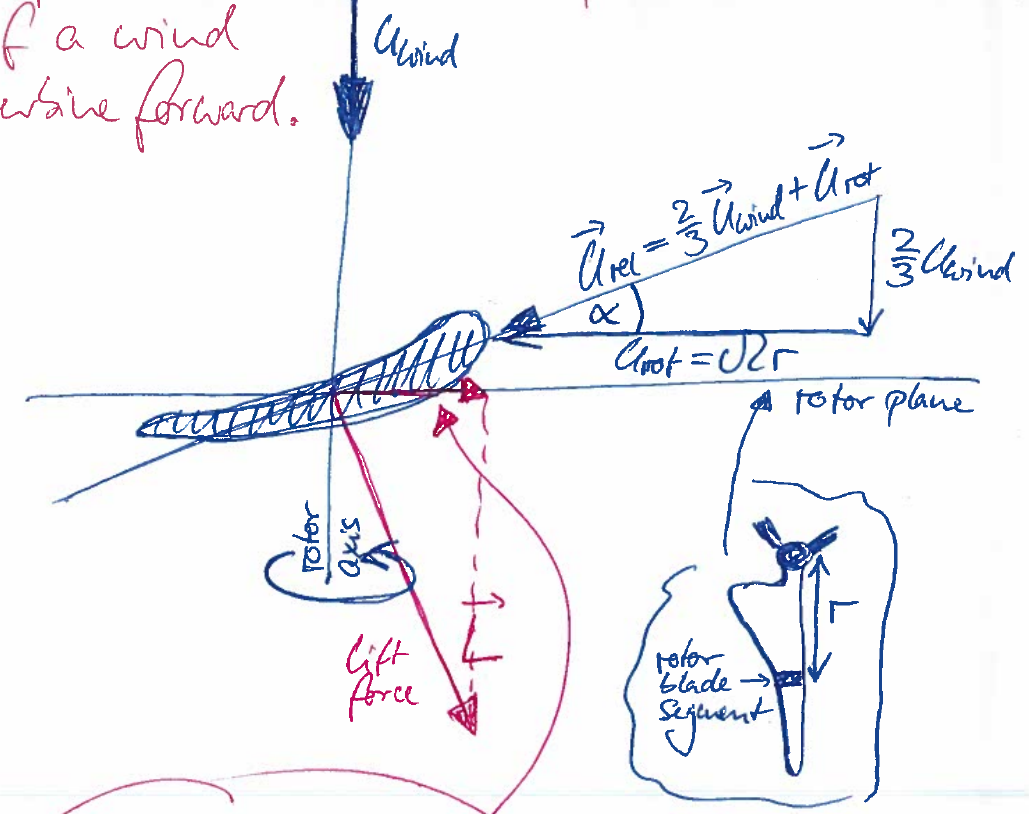
\includegraphics[width=.6\textwidth]{week4/turbine-blade}\\
    \caption{Lift force on the rotor blade of a wind turbine.}
    \label{fig:turbine-blade}
\end{figure}


\subsection[Sailing against the wind]{Sailing against the wind (KCD 14.9)}
People have sailed without the aid of an engine for thousands of years and have known
how to reach an upwind destination. Actually, it is not possible to sail exactly against the
wind, but it is possible to sail at $\approx$ 40-45$^\circ$ to the wind. \fref{fig:sailing-wind} shows
how this is made possible by the aerodynamic lift on the sail, which is a piece of stretched and stiffened
cloth. The wind speed is U, and the sailing speed is V, so that the apparent wind speed relative
to the boat is $U_r$. If the sail is properly oriented, this gives rise to a lift force perpendicular
to U$_\text{r}$ and a drag force parallel to U$_\text{r}$. The resultant force F can be resolved into a driving
component (thrust) along the motion of the boat and a lateral component. The driving
component performs work in moving the boat; most of this work goes into overcoming
the frictional drag and in generating the gravity waves that radiate outward from the hull.
The lateral component does not cause much sideways drift because of the shape of the
hull. It is clear that the thrust decreases as the angle $\theta$ decreases and normally vanishes
when $\theta$ is $\approx$ 40-45$^\circ$ . The energy for sailing comes from the wind field, which loses kinetic
energy after passing the sail.

\begin{figure}[!h]
    \centering
    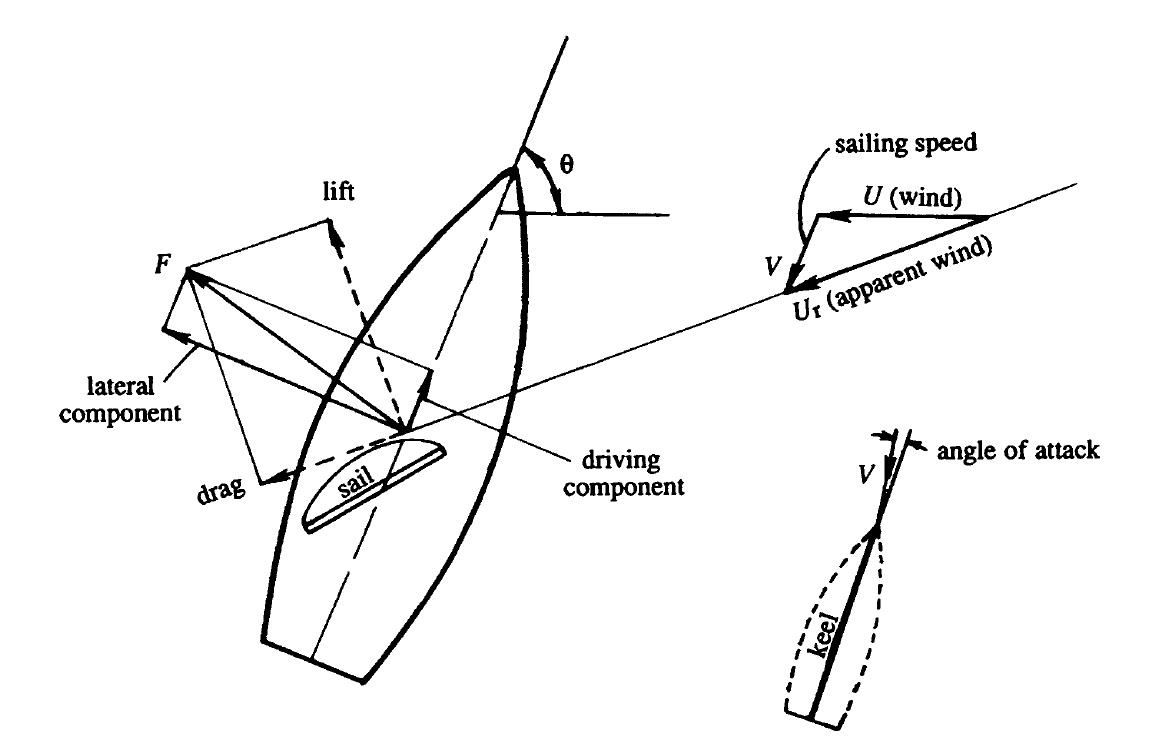
\includegraphics[width=.6\textwidth]{week4/sailing-wind}\\
    \caption{Principle of sailing against the wind. A small component of the sail’s lift pushes the boat forward at an angle $\theta$ < 90$^\circ$ to the wind. Thus by traversing a zig-zag course at angles $\pm\theta$, a sailboat can reach an upwind destination. A sailboat’s keel may make a contribution to its upwind progress too.}
    \label{fig:sailing-wind}
\end{figure}
